\documentclass[11pt]{article}
\usepackage{graphicx}
\usepackage{subcaption}
\usepackage[utf8]{inputenc}
\usepackage[T1]{fontenc}
\usepackage{amsmath}
\usepackage{amssymb}
\usepackage{booktabs}
\usepackage{hyperref}
\usepackage{xcolor}
\usepackage{microtype}
% \usepackage{titlesec}
% \titleformat{\subsubsection}[runin]
%   {\normalfont\normalsize} 
%   {\thesubsubsection}      
%   {1em}                    
%   {}                     
%   []       
% \titlespacing*{\subsubsection}
%   {0pt}                       
%   {1.5ex plus 0.5ex minus 0.2ex} 
%   {0.8ex plus 0.2ex}                 
\usepackage{tikz}

\usetikzlibrary{shapes.geometric, arrows, positioning, fit, backgrounds}
\setcounter{secnumdepth}{3}
\setcounter{tocdepth}{3}
\usepackage[margin=1in]{geometry}
\setlength{\parskip}{0.5em}
\setlength{\parindent}{0em}
\makeatletter
\def\@maketitle{
  \newpage
  \null
  \vskip 2em
  \begin{center}
  \let \footnote \thanks
    {\LARGE \@title \par}
    \vskip 1.5em
    {\large \lineskip .5em
      \begin{tabular}[t]{c}
        \@author
      \end{tabular}\par}
    \vskip 1em
    {\large \@date}
  \end{center}
  \par
  \vskip 1.5em}
\makeatother

\begin{document}

\title{Image Caption Generation With CLIP+GPT-2 Model}
\author{Siyuan Jing and Haonan Wu\\ Boston University \\ siyuan16@bu.edu and whn17@bu.edu}
\date{May 3, 2025}
\maketitle

\begin{abstract}
        This paper presents an image captioning system that combines CLIP with GPT-2.
        We implement a multi-head attention mechanism to effectively bridge between visual and textual modalities. 
        Trained on the MS COCO dataset, 
        our model achieves 94.4\% of human-level consensus quality as 
        measured by CIDEr scores. Our experiments show that the proposed architecture effectively 
        captures both semantic  and syntactic structure in generating natural language descriptions. Additionally, 
        we develop a web-based deployment for real-time captioning
        The results highlight the potential of leveraging pre-trained vision and language 
        models for efficient multimodal understanding with minimal architectural modifications. Codes are avalibale at \url{https://github.com/ChingSsuyuan/Clip_Pro_Caption.git}
\end{abstract}

\section{Introduction}
Image caption generation, the task of recognizing images to generate natural language descriptions, lies at the critical intersection of 
computer vision and natural language processing. 
It plays an important role in a variety of applications, including image retrieval, accessibility for the visually impaired, and automated image content processing.

Recent advances in vision-language models have enabled more accurate and 
fluent caption generation by leveraging large-scale pretraining on aligned image-text pairs 
. These models demonstrate remarkable capabilities in understanding visual content and 
translating it into coherent text descriptions.

Motivated by this progress, we focus our project on replicating a CLIP+GPT-2-based image captioning system, with inspriation from Nukrai et al.\cite{Nukrai2022}. Through this project, we seek to explore and deepen our understanding of 
machine learning, as well as its broader applications in fields such as computer vision and natural language generation.

Our goal is to:
\begin{itemize}
    \item Leverage the pretrained CLIP model to extract semantically rich image embeddings without the need for training a custom vision encoder.
    \item Utilize the generative capabilities of GPT-2 to produce fluent and coherent natural language captions.
    \item Bridge the gap between visual and textual modalities by introducing a projection layer that maps image embeddings into GPT-2's input space.
    \item Enable flexible and data-efficient image captioning, where the visual semantics guide the generation through prefix-based conditioning.
    \item Evaluate the quality of the generated captions using standard metrics such as BLEU and CIDEr, in order to quantitatively assess the model's accuracy and relevance.
\end{itemize}

\section{Background and Related Work}

    \subsection{Contrastive Language-Image Pretraining(CLIP)}
    CLIP from OpenAI is a visual-language model. Instead of relying on 
    task-specific supervised learning, CLIP is trained on a dataset of 400
    million image-text pairs collected from the internet using a contrastive 
    loss function. CLIP consists of two separate encoders: a visual encoder 
    (ResNet) for images, and a text encoder (Transformer) for captions. 
    Its ability to generate rich, semantically meaningful image 
    embeddings makes CLIP a powerful foundation for our systems and 
    an ideal visual component in our CLIP+GPT-2 image captioning pipeline. 
    For example, according to Mokady et al.\cite{Mokady2021}, it mentioned that the visual encoding capability of 
    CLIP can be used to embed and project the generated images into the input 
    space of GPT-2 to generate prefixes, which helps the final caption generation of GPT-2. Inspired by this article, we decided to study the CLIP architecture and implement related deployments.

    \subsection{Generative Pre-trained Transformer 2 (GPT-2)}
    GPT-2 is a large-scale language model based on the Transformer 
    decoder architecture proposed by Radford et al.\cite{Radford}. 
    According to the paper, Transformer completely replaces the traditional RNN or 
    CNN structure with self-attention, which is more efficient and accurate when processing 
    long sequence dependencies. Therefore, we consider implementing the transformer 
    structure as our decoder of the whole pipeline. Unlike the traditional 
    Transformer, which contains both encoder and decoder components, 
    GPT-2 uses only a decoder. This design enables the model to predict the next token based solely on previously generated tokens, 
    making the generated text semantically relevant and well suited for text generation tasks such as image captioning.
    
    \subsection{Multi-Head Attention Mechanism}
    Inspired by the \textit{``Attention Is All You Need''} paper 
    \cite{vaswani2017attention}, we employ a multi-head attention 
    mechanism as a cross-modal connector between the CLIP image embedding
    and the GPT-2 language model. Instead of using a linear layer to directly 
    project the CLIP features into the GPT-2 embedding space, we employ an 
    attention mechanism that enables the model to selectively focus on 
    different aspects of the visual features when generating each token 
    in the caption, making the generated tokens more consistent with the 
    image information. Multi-head Attention network allows the model to 
    learn how different regions in the image affect language production.

We compare these advanced approaches of image caption generation to understand its 
advantages and limitations, and implement these methods in the process of model training to get our own model.
\pagebreak
\section{Methodology}

\subsection{Implementation Details}
\textbf{Detail of Implementation and pipeline:} This is the pipeline of 
our entire training process, which mainly includes multiple steps: 
image input, feature extraction and encoding, feature processing, 
feature decoding, model training and error evaluation. We will also 
introduce the optimization we used.

    \begin{figure}[h]
    \centering
    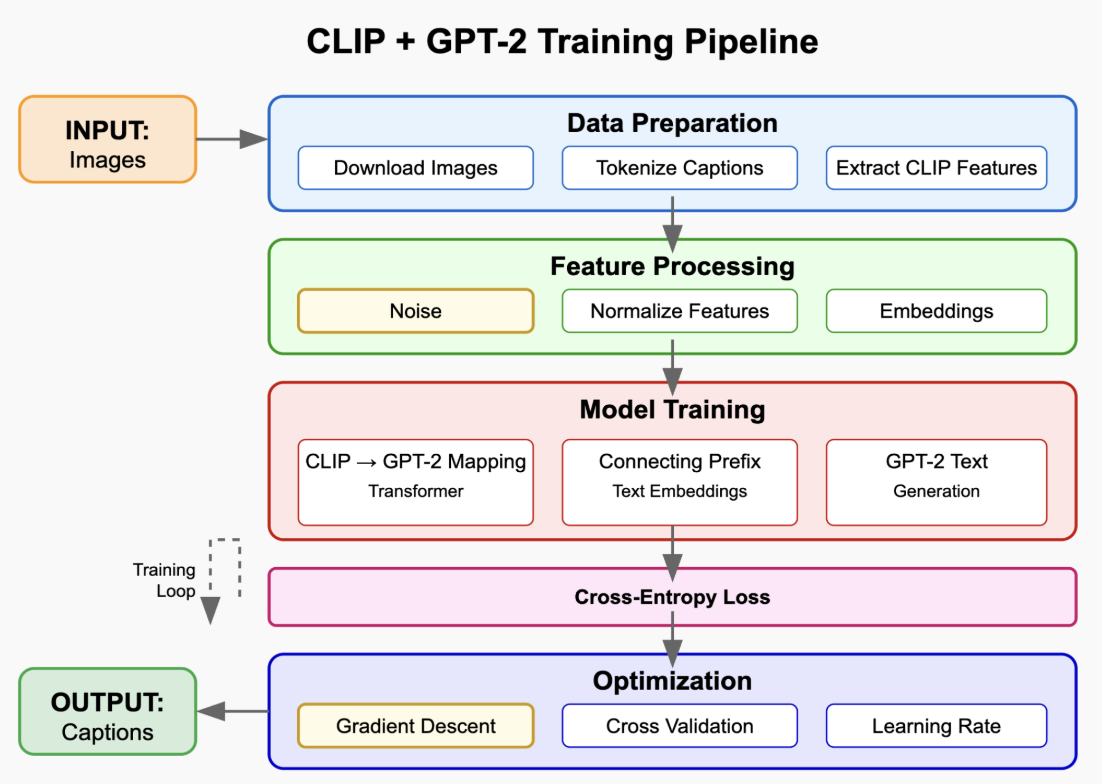
\includegraphics[width=0.8\textwidth]{figure1.png}
    \caption{CLIP+GPT-2 Training Pipeline}
    \label{fig:architecture}
    \end{figure}

    \subsubsection{DataSet}

    We utilize the MS COCO dataset \cite{COCO}for training and evaluation, 
    MS COCO (Microsoft Common Objects in Context) 
    is a large-scale image recognition, segmentation, 
    and annotation dataset that is widely used in research 
    in the field of computer vision, especially in tasks 
    such as image captioning, object detection, and semantic 
    segmentation. It contains 330K images with 5 captions each. 
    We will split our dataset into three parts: 80\% training, 10\% validation, 10\% testing.

    \subsubsection{Data Preparation}
    After we get the original CLIP embedding, we will normalize it for better training performance. In the actual training process, 
    we found that the trained model may be overly sensitive to some features of some pictures, 
    so we add some noise to 10\% of the feature information of each picture to improve generalization ability and reduce overfitting. 
    These embeddings can then be projected into the GPT-2 space for training.
    \subsubsection{Feature Process}
    After we get the original CLIP embedding, 
    we will normalize it for better training performance. 
    In the actual training process, we found that the 
    trained model may be overly sensitive to some 
    features of some pictures, so we add some noise to 
    10\% of the feature information of each picture to 
    improve generalization ability and reduce overfitting. These embeddings can then be projected into the GPT-2 space for training.

    \subsubsection{Model training}
    Next, we use a multi-layer Transformer to map the 
    CLIP embedding to the word embedding space of GPT-2 
    to create a prefix. This prefix is then concatenated 
    with the tokenized caption, which is generated in the data preparation stage,  
    to form the whole input sequence for GPT-2. After receiving these input sequences, 
    the GPT-2 model is trained for a set rounds of training loop to generate the caption of the corresponding image based on the given prefix and token.

    \subsubsection{Optimization method}
    For the weight matrix obtained after each round of training, we use sub-gradient descent 
    to adjust the weights. Additionally, during the entire training process, we use cross-validation to 
    find the optimal solution for multiple hyperparameters in the model, and reasonably control the learning rate to obtain better training results.
\subsection{Loss and objective function for training process}

We use the cross-entropy loss function to measure the difference between the caption generated by the model and the ground-truth captions. The loss function is defined as:

\textbf{The Cross-entropy Loss Function:}
\begin{equation}
\text{Loss} = -\sum_{t=1}^{T} \log P_{\text{GPT-2}}(w_t \mid w_{<t}, \text{prefix})
\end{equation}

Where:  
\begin{itemize}
    \item $T$ — the total number of tokens (words) in the caption  
    \item $w_t$ — the actual word at position $t$ in the ground-truth caption  
    \item $w_{<t}$ — the sequence of all previous words before time step $t$  
    \item $\text{prefix}$ — the mapped image feature vector used to condition the generation  
    \item $P_{\text{GPT-2}}(w_t \mid w_{<t}, \text{prefix})$ — the probability assigned by GPT-2 to word $w_t$ given previous words and the image prefix
\end{itemize}

This loss encourages the model to assign a higher 
probability to the correct next word at each time step. 
Minimizing the cross-entropy loss over the training data 
helps the model generate captions that are more fluent 
and accurate.

\pagebreak
\textbf{The Objective Function in Maximum Likelihood Estimation:}

\begin{equation}
\hat{\theta} = \arg\min_{\theta} -\sum_{i=1}^{N} \sum_{t=1}^{T_i} \log P_\theta(w_t^{(i)} \mid w_{<t}^{(i)}, \text{prefix}^{(i)})
\end{equation}

Where:
\begin{itemize}
    \item $\theta$ — model parameters, including GPT-2 weights and the parameters of the prefix mapping network  
    \item $N$ — the total number of training samples (image-caption pairs)  
    \item $T_i$ — the number of tokens in the $i$-th caption  
    \item $w_t^{(i)}$ — the $t$-th word in the $i$-th ground-truth caption  
    \item $w_{<t}^{(i)}$ — all previous words before position $t$ in the $i$-th caption  
    \item $\text{prefix}^{(i)}$ — the mapped image features for the $i$-th image
\end{itemize}

This objective function aims to find the parameter set $\hat{\theta}$ that minimizes the total negative log-likelihood 
across the training dataset. During training, the model updates $\theta$ using optimization 
techniques such as gradient descent, guided by cross-validation to avoid overfitting and improve generalization.
\begin{figure}[h]
    \centering
    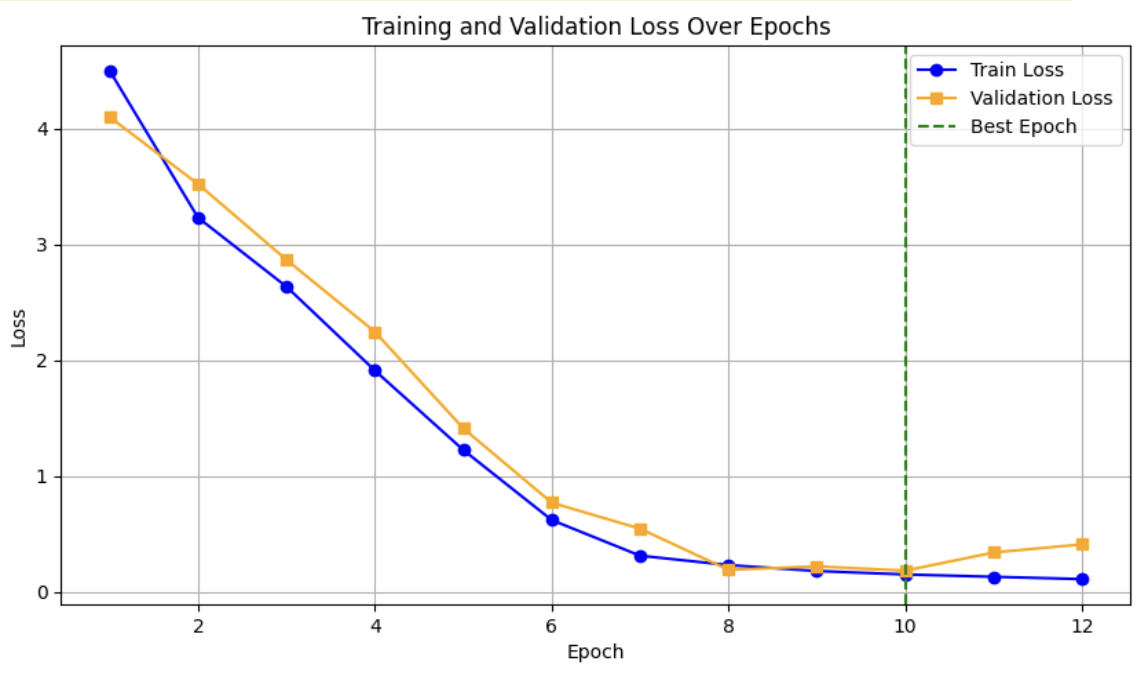
\includegraphics[width=0.8\textwidth]{f2.png}
    \caption{Training and validation loss over epochs}
    \end{figure}
\pagebreak
\section{Experiments and Results}
\subsection{Training Details}
We train our model using these hyperparameter after cross-validation:
\begin{itemize}
  \item Prefix length: 40
  \item Transformer layers: 8
  \item Number of epochs: 12
  \item Noise rate: 10\%
  \item Optimizer: Adam with a learning rate of $5 \times 10^{-5}$
\end{itemize}

We conduct experiments on:
\begin{itemize}
  \item \textbf{COCO Image Dataset:}
  
  Training set: 80, 000 images with 5 captions per image.

  Validation set: 2,000 images.
  
\end{itemize}

\subsection{Evaluation Metrics}
After completing model training, we need to evaluate the quality of generated captions to assess the effectiveness of our approach. Therefore, we adopt two widely used 
automatic evaluation metrics in the field of image captioning: BLEU and CIDEr.
\begin{itemize}
    \item \textbf{Bilingual Evaluation Understudy }
    
    BLEU is a baseline evaluation 
    metric of our model that measures the accuracy of n-gram overlap between predicted captions 
    and one or more real captions\cite{Papineni}. It emphasizes syntactic similarity and is particularly sensitive to exact word 
    matching and word order. However, this criterion lacks semantic awareness and often penalizes correct words due to different word position information.

    \item \textbf{Consensus-based Image Description Evaluation}
    To address the shortcomings of the above evaluation method, we also chose the CIDEr
     (Consensus-based Image Description Evaluation) \cite{vedantam2015cider}
     evaluation metric, which is designed specifically for image 
     captioning. It uses a TF-IDF weighted n-gram model to evaluate how well the 
     generated captions match the manually generated captions. This design increases the 
     weights of rare but informative words (e.g., nouns, verbs, adjectives, etc., which often contain unique image information) 
     while reducing the weights of function words such as articles (a, the), quantifiers (some, many), and prepositions (in, on, at).
\end{itemize}

\pagebreak
\subsection{Generation Results}
\textbf{Prediction Scores:}

We compute BLEU and CIDEr on our test set and compare the original captions' scores with our outputs:
\begin{figure}[h]
    \centering
    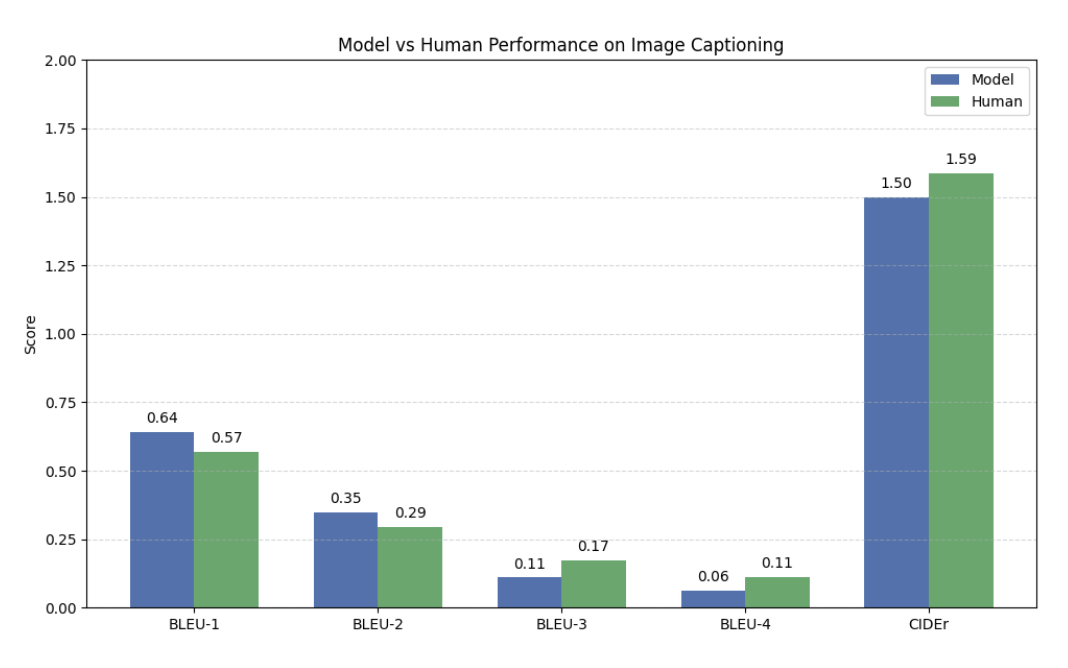
\includegraphics[width=0.8\textwidth]{f3.png}
    \caption{Model vs Human Performance on Image Captioning}
    \end{figure}
\begin{itemize}
    \item Human captions show better performance on longer word sequences, indicating more natural grammatical structure.
    \item The CIDEr score shows our model can achieve 94.4\% of human-level consensus quality.
\end{itemize}
\pagebreak
\textbf{Web-based Deployment for Real-time Captioning}

We design and deploy a website to realize our model
function. The website is able to upload images and load the pre-trained model to generate 
captions within 10 seconds.

\begin{figure}[h]
    \centering
    \begin{subfigure}[b]{0.45\textwidth}
        \centering
        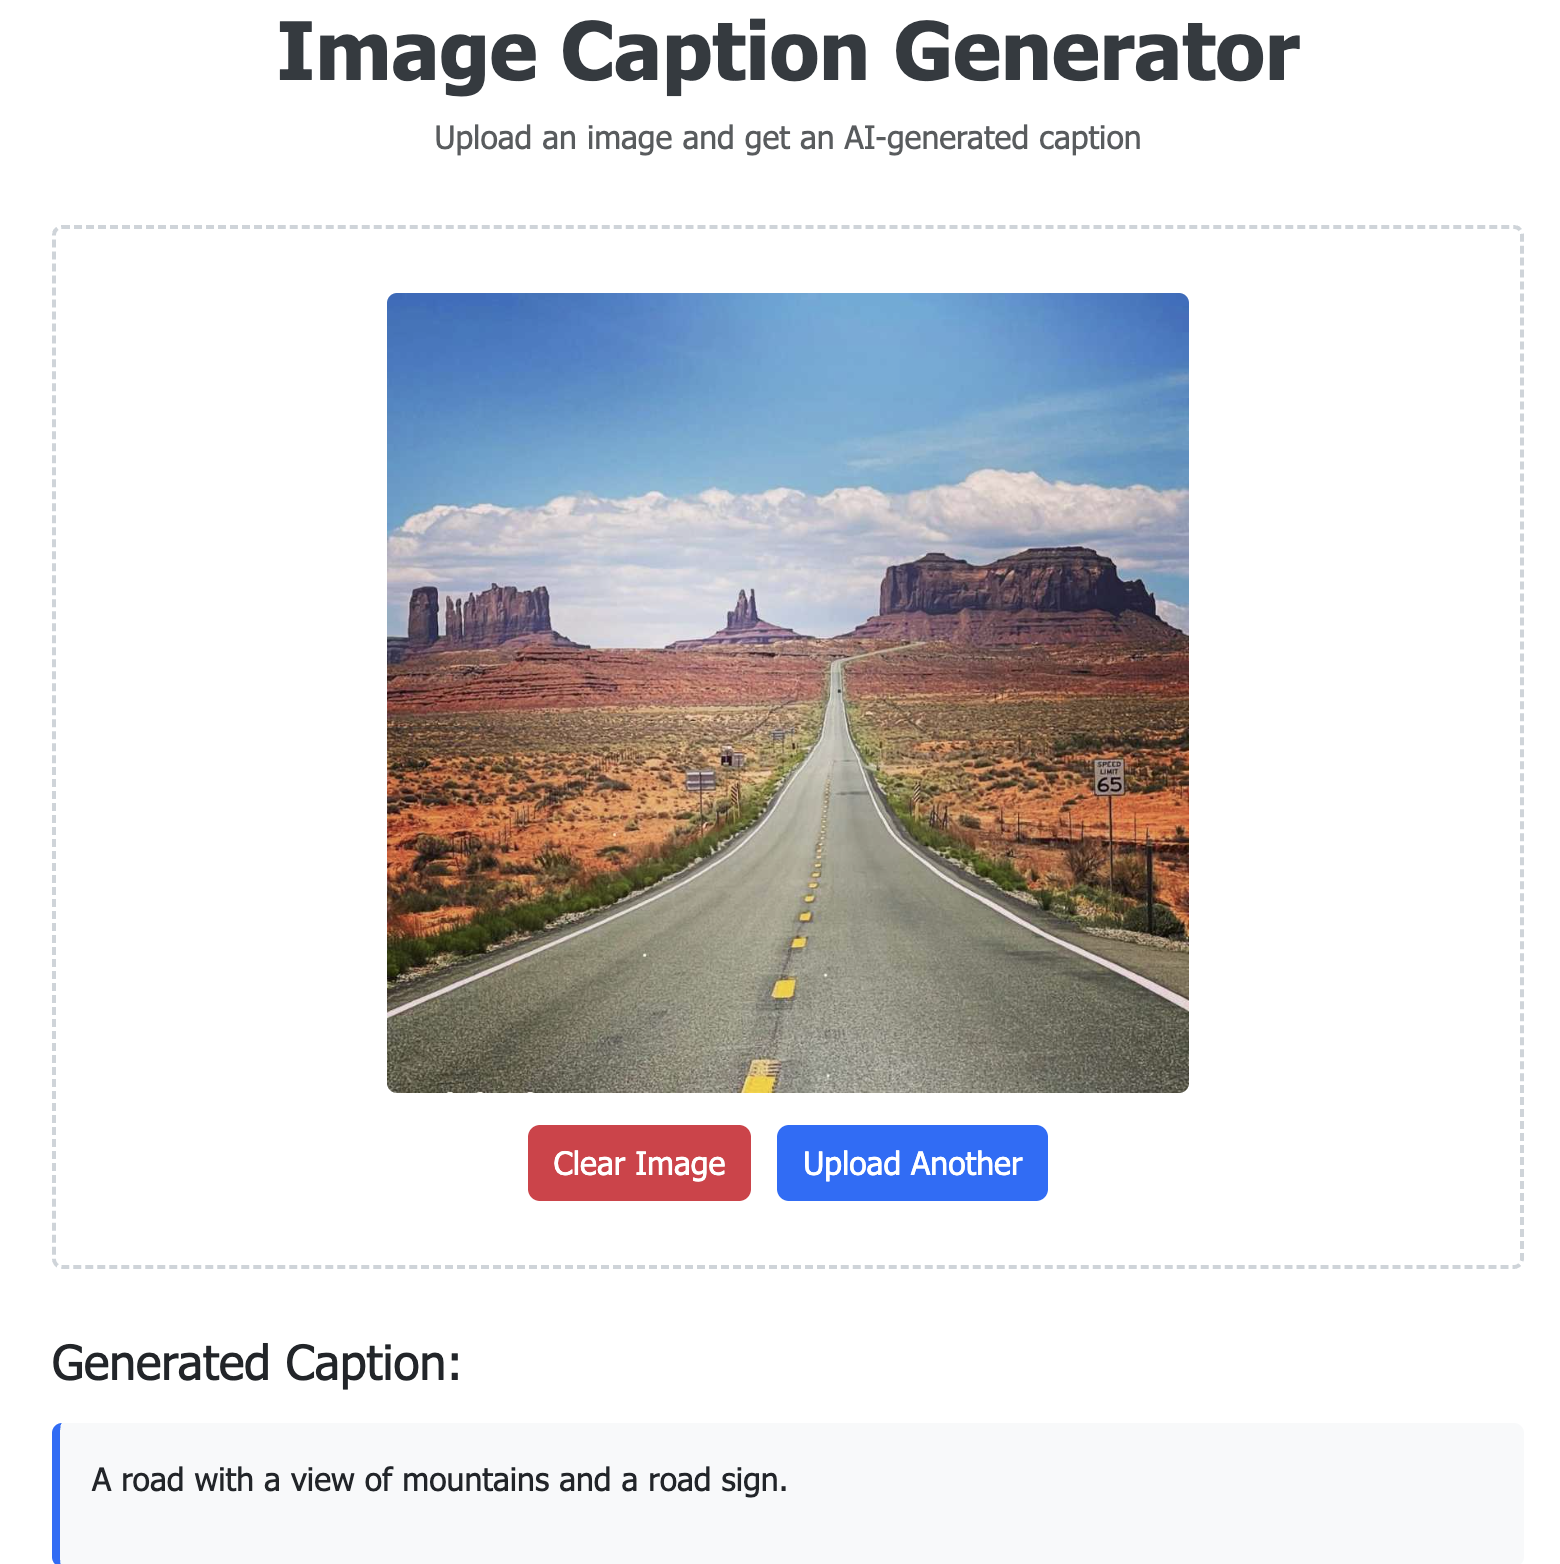
\includegraphics[width=\textwidth]{F4.png}
        \caption{Example 1}
        \label{fig:upload}
    \end{subfigure}
    \hfill
    \begin{subfigure}[b]{0.43\textwidth}
        \centering
        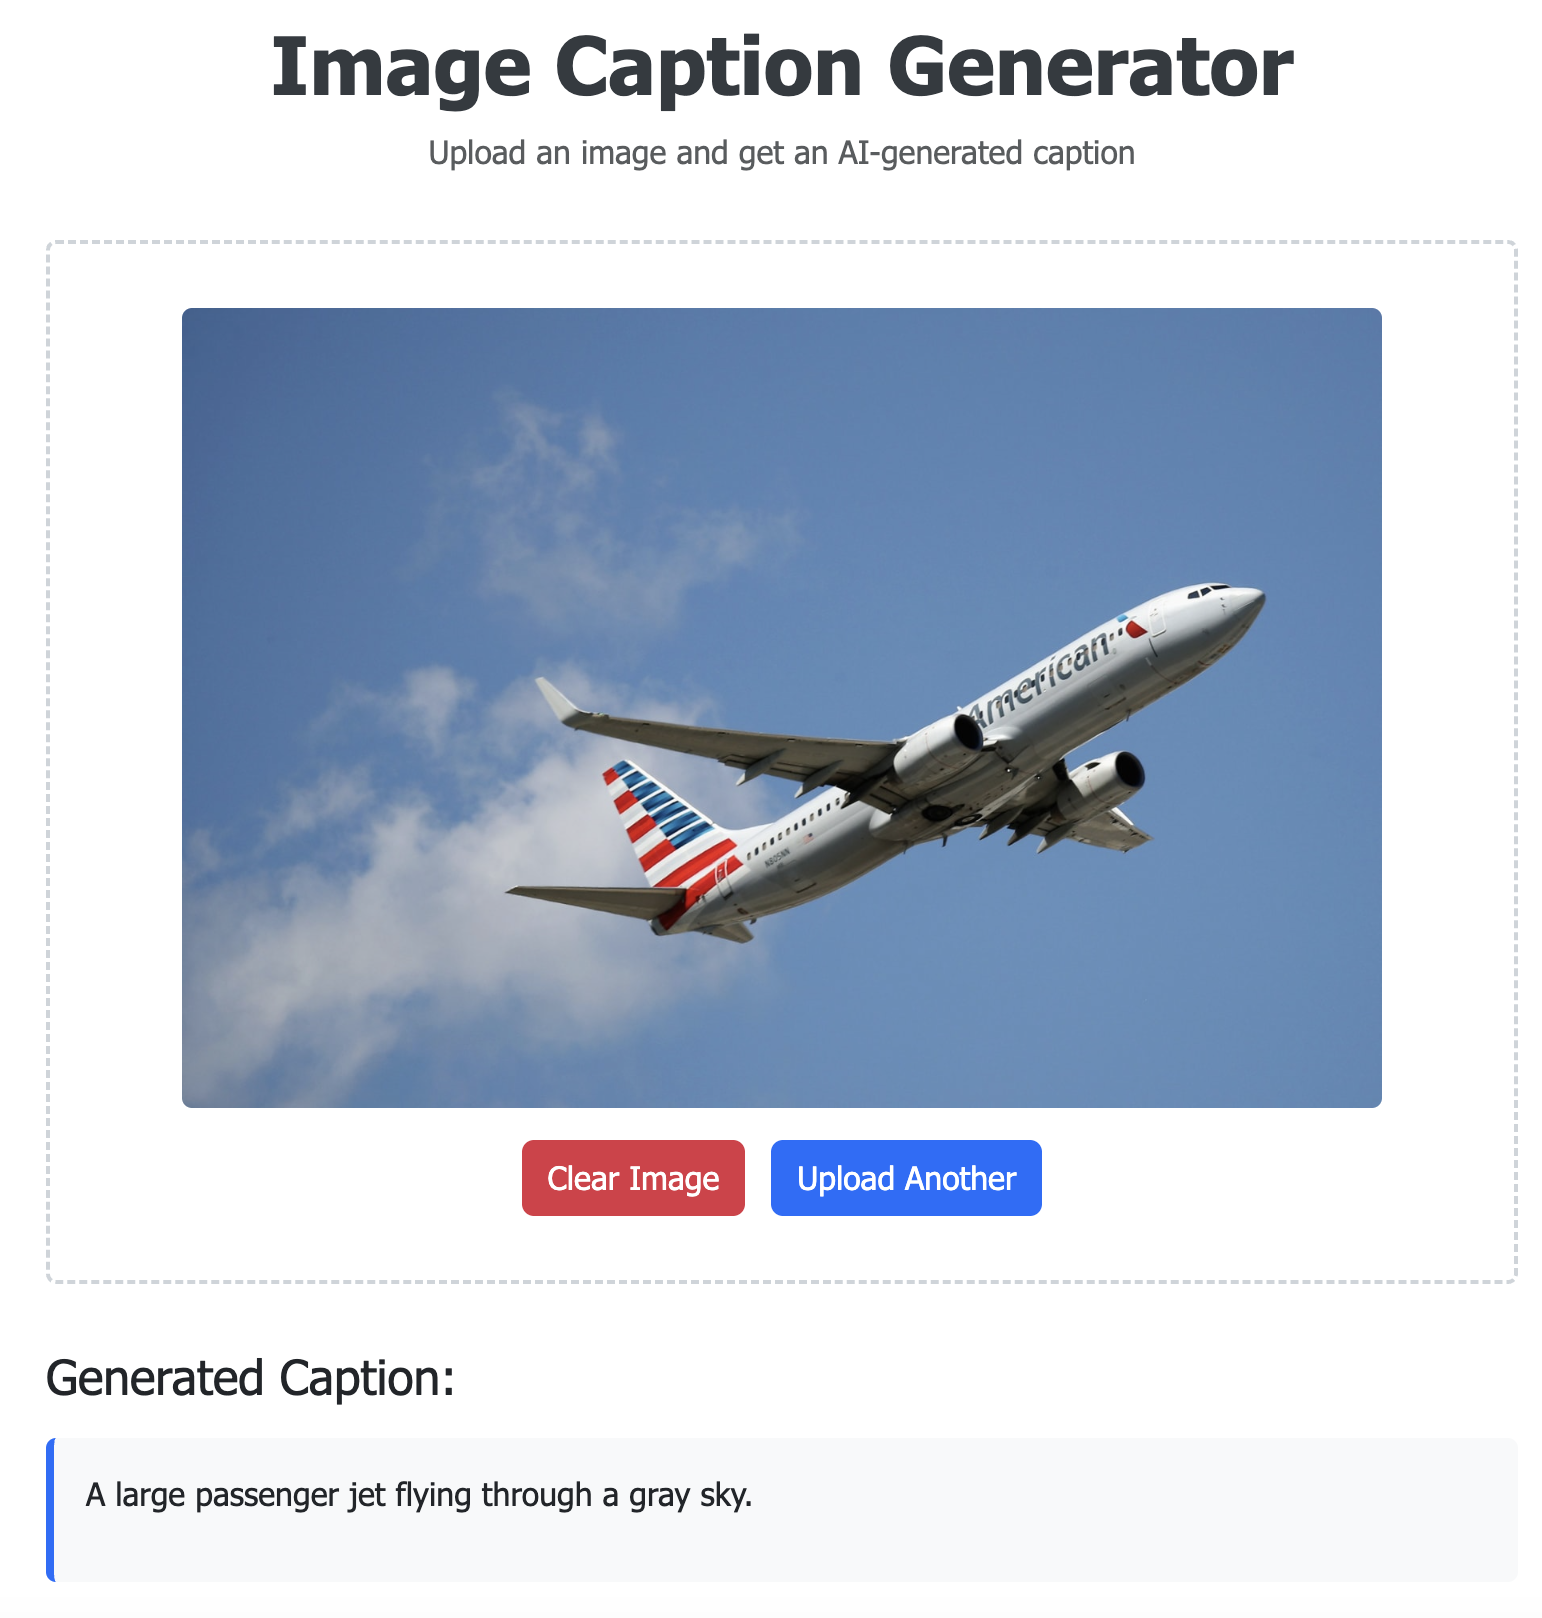
\includegraphics[width=\textwidth]{F5.png}
        \caption{Example 2}
        \label{fig:caption}
    \end{subfigure}
    \caption{Web demo of our deployed model: From image upload to automatic caption generation}
    \label{fig:web_demo}
\end{figure}

\section{Discussion}

\subsection{Key Findings}
\begin{itemize}
    \item Automated organization of visual content: 
    
    Our model demonstrates strong automatic organization 
    capabilities for visual content, especially when dealing 
    with a large number of unlabeled images. By generating 
    relevant and informative captions, the system can group 
    images without manual annotation.

        \item Effective CLIP-to-GPT-2 Mapping:
  
    The key design of our entire model is the multi-head 
    attention mechanism used to connect CLIP visual embedding
    and GPT-2 language model input. Unlike simple linear projection, 
    the multi-head attention mechanism enables the model to learn 
    multiple semantic alignment patterns between image features and 
    different dimensions of generated captions. Test results show 
    that the implementation of this mechanism can generate more 
    accurate captions that reflect the details of image semantics.

    \item Noise Injection Boosts Generalization:
    We observe that adding small Gaussian noise into CLIP embeddings 
    during training improves the model's generalization across 
    different image inputs. This regularization technique helps 
    the mapping module avoid overfitting to specific embedding 
    patterns and encourages the model to generate captions that
    are both accurate and diverse. Result shows that noise
    improves both BLEU and CIDEr scores, indicating improved
    robustness and semantic coverage of caption generation.
    
\end{itemize}

\subsection{Future Work}
In future work, we plan to expand the test 
dataset to cover more diverse and challenging images to 
more robustly evaluate the generalization ability of our model. 
In addition, we can try to study and combine more powerful visual 
language models (such as CLIP ViT-L or GPT-3 variants) to achieve 
stronger semantic alignment capabilities.

\section{Conclusion}
In this project, we implemented an image captioning 
system by combining the powerful visual encoding capabilities 
of CLIP and the generative language capabilities of GPT-2. By 
introducing a mapping module based on a multi-head attention 
mechanism, we effectively reduced the gap between visual and 
textual modalities, enabling the generation of fluent and 
semantically relevant captions. We further enhanced the 
generalization ability of the model by adding noise during training, and selected appropriate loss functions and objective functions for training. Finally, evaluations using BLEU and CIDEr metrics confirmed the effectiveness of our model, especially in capturing human-written semantics, with the CIDEr score reflecting its excellent performance.


\pagebreak
\begin{thebibliography}{99}
    \bibitem{Nukrai2022}
    Nukrai, D., Mokady, R., \& Globerson, A. (2022). Text-Only Training for Image Captioning using Noise-Injected CLIP. https://doi.org/10.48448/n7sq-p557
    
    \bibitem{Mokady2021}
    Mokady, R., Hertz, A., \& Bermano, A. H. (2021). ClipCap: CLIP Prefix for Image Captioning. http://arxiv.org/abs/2111.09734
    
    \bibitem{Radford}
    Radford, A., Wu, J., Child, R., Luan, D., Amodei, D., \& Sutskever, I. (2019). ``Language Models are Unsupervised Multitask Learners.'' OpenAI Technical Report.

    \bibitem{vaswani2017attention}
    Vaswani, A., Shazeer, N., Parmar, N., Uszkoreit, J., Jones, L., Gomez, A. N., Kaiser, Ł., \& Polosukhin, I. (2017). ``Attention is all you need.'' 
    Advances in Neural Information Processing Systems, 30.

    \bibitem{COCO}
    Xinlei Chen, Hao Fang, Tsung-Yi Lin, Ramakrishna Vedantam, Saurabh Gupta, Piotr Dollár, and C Lawrence Zitnick. 2015. Microsoft coco captions: Data collection and evaluation server. arXiv preprint arXiv:1504.00325.
    
    \bibitem{Papineni}
    Papineni, K., Roukos, S., Ward, T., \& Zhu, W. J. (2002). ``BLEU: a method for automatic evaluation of machine translation.'' ACL 2002.
    
    \bibitem{vedantam2015cider}
    Vedantam, R., Lawrence Zitnick, C., \& Parikh, D. (2015). ``CIDEr: Consensus-based image description evaluation.'' CVPR 2015.
    
    \end{thebibliography}

\end{document}